\chapter{Projeto e Implementação}

Tendo em vista todos os pontos observados anteriormente, é levantado o perfil da arquitetura do sistema, como pode ser visto na figura a seguir. O projeto foi segmentado em camadas de acordo com a tecnologia sendo implementada (linhas pretas pontilhadas).

Também foram designados microsserviços principais que distinguiam o caminho crítico que desejamos obter. Cada um desses foi descrito neste capítulo.

\begin{figure}[ht]
  \centering
    \caption{Diagrama esquemático da arquitetura}
    \includegraphics[scale=0.7]{arquitetura}
  \centerline{\small{Fonte: autores}}
\end{figure}
\FloatBarrier

Todo código elaborado pelos autores com relação a cada projeto é acessível no link da organização do repositório do grupo\cite{github}.

\section{Módulo Do Target}

Essa etapa engloba possibilitar a comunicação unidirecional de cada dispositivo nos animais (\emph{target}). Essa comunicação foi feita através da emissão em \emph{broadcast} de pacotes utilizando Sub-1GHz, que trabalha a frequência de 868MHz, com o protocolo proprietário da TI, chamado \emph{EasyLink Proprietary RF}.

Além disso, era necessário que o \emph{target} tivesse um ciclo de \emph{sleep}, de forma a controlar a taxa de transmissão do sinal, reduzindo a energia consumida por cada dispositivo. Estudos foram feitos para se decidir qual a melhor estratégia de implementação.

\subsection{Comunicação unidirecional}

Para tal, o módulo padrão de transmissão (Tx) disponibilizado pela TI foi estudado e modificado para que o pacote enviado contivesse o Identificador (ID) de cada animal - que ficou codificado de maneira pré definida em cada \emph{SensorTag}.

Esse módulo cria uma \emph{task} para a execução da tarefa de emissão dos pacotes cujo \emph{payload} e endereço de destino podem ser configurados. Como só era desejado o ID do macaco e a intensidade do sinal, o \emph{payload} foi constituído somente por um único \emph{byte} contendo a primeira informação. Tendo isso em vista, é compreensível que seria possível inserir no mesmo \emph{payload} demais informações relativas aos animais através dos sensores em cada placa.

Regular a potência do sinal é interessante uma vez que tanto o alcance do sinal quanto a precisão observada no RSSI variam. Adotamos uma intensidade arbitrária de 12 dB para a qual observamos que para cerca de 30 metros o ponto de acesso ainda recebia resposta.

\subsection{Temporização}

Para controle do ciclo de envio e \emph{sleep} do módulo \emph{target}, foram pesquisadas três principais estratégias:

\begin{enumerate}
  \item Utilização de um periférico do microcontrolador do \emph{SensorTag} do tipo \emph{timer}, para determinação do período de sleep através de seu contador;
  \item Por meio de uma pausa na tarefa do sistema operacional que está executando a transmissão de pacotes;
  \item Ou alterando-se uma constante da estrutura de pacotes.
\end{enumerate}

A \emph{Texas Instruments} permite que o controle dos periféricos dos módulos utilizados seja feito por meio do uso de \emph{API}s específicas de seus \emph{drivers}. No caso do \emph{timer}, é possível utilizar a referência da biblioteca GPTimerCC26XX.h \cite{gptimer}. Ela contém funções básicas de operação do \emph{timer}, como init(), start(), stop() e callback().

Para utilização do \emph{timer}, é necessário também que se configure seus parâmetros. Alguns deles, mais essenciais, são:

\begin{itemize}
	\item Modo (\emph{One-shot}, Modulação por largura de pulso, periódico, dentre outros);
	\item Tamanho máximo do contador (pode ser de 16 ou 32 bits);
	\item Valor até o qual o \emph{timer} deve contar;
	\item Função de retorno;
\end{itemize}

Todos esses parâmetros são referenciados no datasheet do microcontrolador \cite{datasheet} e na referência da biblioteca do \emph{driver} \cite{gptimer}. No contexto do \emph{SensorTag} e deste projeto, o \emph{timer} pode ser configurado para funcionar de maneira periódica e a transmissão de mensagens ser incluída em sua função de \emph{callback}.

O cálculo da periodicidade do \emph{timer} deve ser feita levando-se em conta a sua frequência de atualização, lembrando que, em uma descrição simples, o funcionamento do \emph{timer} consiste em contar de 0 até o valor especificado em seus parâmetros. O memorial de cálculo encontra-se no Apêndice 4.

Boa parte dos exemplos de uso de periféricos providos pela TI incluem criação de tarefas. Conforme mencionado no início do capítulo 6, utilizou-se primariamente um dos exemplos fornecidos pela TI para operação do módulo de \emph{target}. Uma solução mais simples do que configurar o \emph{timer} (e possivelmente menos custosa) seria utilizar a função Task\texttt{\char`_}Sleep(nticks) \cite{task-modules}. O que esta função faz em essência é bloquear a tarefa pelo tempo definido em nticks, o qual é medido em microssegundos e tem como referência o próprio \emph{clock} do sistema (48MHz \cite{datasheet}).

Uma última estratégia seria utilizar um dos parâmetros da própria estrutura de mensagens de trasmissão do protocolo utilizado \cite{forum-easylink}. Tal parâmetro é EasyLink\texttt{\char`_}ms\texttt{\char`_}To\texttt{\char`_}RadioTime e é medido em microssegundos, como seu nome sugere \cite{easylink}. Seria uma alternativa às duas últimas mencionadas, porém, há pouca informação sobre seu tamanho máximo e há relatos de outros usuários da API sobre problemas em seu uso por este motivo.

\subsection{Eficiência Energética}

Para efeito de preservação da bateria escolheu-se realizar a transmissão a cada 5 segundos de maneira a manter o aspecto de atualização em tempo real. Tal valor pode ser configurado facilmente alterando-se uma das variáveis contidas nas estratégias de temporização mencionadas anteriormente (loadVal para o \emph{timer}, nTicks para Task\texttt{\char`_}Sleep() e EasyLink\texttt{\char`_}ms\texttt{\char`_}To\texttt{\char`_}RadioTime para a estrutura dos pacotes). Esta mudança deve ser feita caso seja julgada interessante uma maior economia de energia em troca de desempenho.

\section{Módulo Do Ponto De Acesso}

Cada ponto de acesso é responsável pela leitura e armazenamento dos dados correspondentes aos pacotes enviados pelos \emph{targets}. Assim, para cada pacote recebido é possível identificar a intensidade do sinal, que é armazenada em um vetor de tamanho fixo junto com o ID do macaco.

Uma vez que o vetor estiver completo, o ponto de acesso cria e envia pacotes de maneira similar a como é feita pelos \emph{targets}, mas com endereço de destino distinto, por exemplo 0xBB.

Para isso, foi desenvolvido um projeto composto por ambos os módulos padrão de leitura (Rx) e transmissão (Tx). O módulo de leitura é configurado para que passem pelo filtro somente pacotes cujo endereço de destino seja igual ao dos enviados pelo \emph{target}, por exemplo 0xAA.

\section{Módulo Central}

A mediação da comunicação entre o ponto de acesso (\emph{SensorTag}) e o controlador (\emph{Raspberry Pi}) deve ser feita através do nó denominado Central implementado por um \emph{SensorTag} conectado por UART ao controlador.
Este componente terá a função de receber os pacotes filtrados pelo endereço de destino configurado pelos pontos de acesso e repassar as informações por conexão serial para o controlador.

Para isso, analogamente ao realizado nos demais componentes, foi desenvolvido um projeto composto por ambos os módulos padrão de leitura (Rx) e transmissão serial UART disponibilizados pela TI. Essa composição foi feita criando uma \emph{thread} para cada módulo utilizando \emph{buffers} duplos, de forma que cada tarefa trabalhasse paralelamente em um \emph{buffer} individual.

O tamanho dos \emph{buffers} foi dimensionado para abrigar 32 medidas, considerando a memória máxima da placa e, ao mesmo tempo, a não sobrecarregar a comunicação serial com o controlador, que depende da interrupção dessa comunicação para escrever no banco. O módulo UART é configurado para atuar a taxa de transmissão de 115200 bits por segundo sem paridade.

\subsection{Integração dos pontos de acesso e target}

Definidos os módulos de \emph{target}, ponto de acesso e ponto central, o seu funcionamento conjunto é ilustrado conforme o diagrama da Figura 7, conjuntamente com as principais funções de cada módulo.

O projeto Simio-Tx representa o comportamento do módulo \emph{target} que é responsável por emitir pacotes com a identificação do macaco em que está instalado (pacote 1) e possui a função de Task\texttt{\char`\_}Sleep() para diminuir o consumo energético.

AP\texttt{\char`\_}Peripheral\texttt{\char`\_}RxTx é o projeto que implementa o funcionamento dos pontos de acesso. Ele atua concomitantemente como receptor e transmissor: recebe o ID do macaco monitorado em diversos horários até que o \emph{buffer} de mensagem a ser enviada ao ponto central esteja cheio, então envia as informações que recebeu conjuntamente com o horário calculado e o parâmetro de RSSI (usado no \emph{Raspberry Pi} para fazer o cálculo da distância).

Já o projeto AP\texttt{\char`\_}central\texttt{\char`\_}RxUART recebe as informações de monitoramento dos três pontos de acesso, e assim as envia por UART para o \emph{Raspberry Pi}.

\begin{figure}[ht]
  \centering
    \caption{ Funcionamento conjunto dos nós do sistema.}
    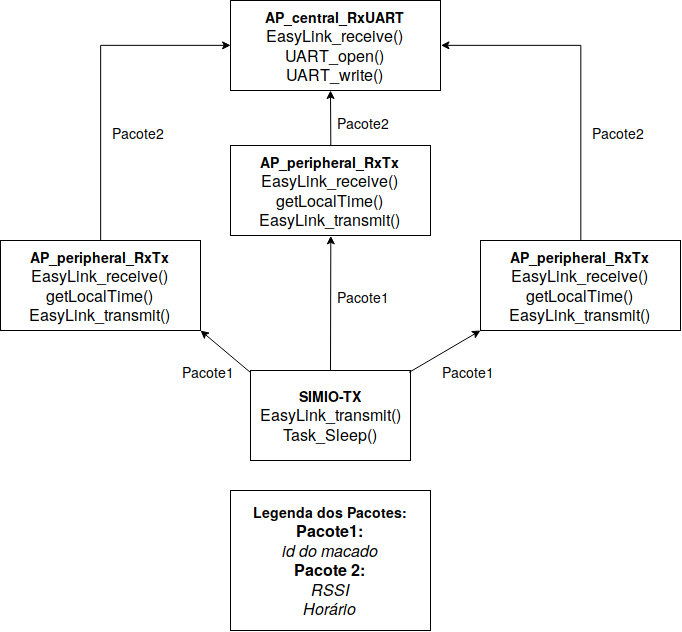
\includegraphics[scale=0.65]{sensortag-arquitetura}
  \centerline{\small{Fonte: autores}}
\end{figure}
\FloatBarrier

\section{Módulo Do Controlador}

Como módulo controlador escolheu-se uma placa \emph{Raspberry Pi} que deve estar conectada ao módulo central. Para evitar demais interferências do ambiente e com isso demais gargalos na comunicação, os dois módulos se comunicam de forma serial através de UART. No módulo controlador isso se dá pela biblioteca "serial" em python.

Ao receber as informações, o controlador deve formatar os dados das distâncias e \emph{timestamps} de cada medida tomada. Neste momento os valores de RSSI recebidos devem ser convertidos em distâncias em metros através do equacionamento obtido no item 2.4 deste documento e os \emph{timestamps} são ajustados para o tempo ao qual o controlador está conectado. Além disso, os valores da mensagem são checados para determinar se a mensagem está completa e coerente, ou seja, se não houve perda de dados durante os envios anteriores e é descartada em caso negativo.

Após receber e processar os dados o controlador deve enviá-los para o banco de dados no servidor. Já que não há problemas de armazenamento no controlador ele deve aguardar para enviar as informações para o banco assim que não houver mensagens sendo recebidas na conexão serial, já que seria demasiadamente custoso para o \emph{SensorTag} guardar e transmitir suas leituras.

A solução escolhida foi o uso da biblioteca \emph{MySQLdb} em \emph{Python}, com a qual os dados são inseridos diretamente no banco de dados utilizando \emph{SQL queries}. Como é boa prática, as mensagens são analisadas antes que de serem enviada para garantir que os dados se encaixam no que foi definido no banco. Caso haja problemas na conexão com o servidor elas são armazenadas no controlador até que ele consiga se reconectar.

O comportamento previamente descrito é esquematizado pela máquina de estados a seguir:

\begin{figure}[ht]
  \centering
    \caption{Máquina de estados representando o funcionamento do módulo controlador}
    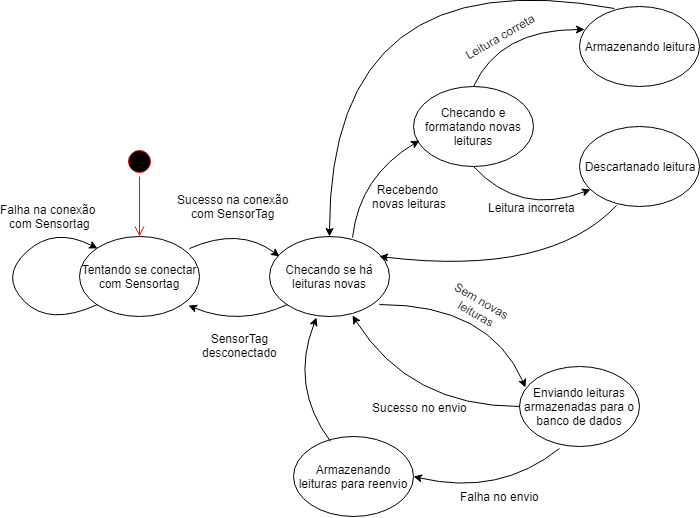
\includegraphics[scale=0.65]{estados-raspberry}
  \centerline{\small{Fonte: autores}}
\end{figure}
\FloatBarrier

\section{Banco De Dados}

O modelo desenvolvido é relativamente simples e envolve somente os objetos físicos do contexto, de forma que fique claro que são mapeados: o \emph{target}, o ponto de acesso e a distância entre eles.

Pelo lado da segurança do sistema, foi utilizado um modelo padrão do \emph{Spring Security} que mapeia o usuário e suas permissões como pode ser visto no diagrama de classes a seguir.

\begin{figure}[ht]
  \centering
    \caption{Diagrama de classes gerado pela ferramenta de engenharia reversa do MySQL}
    \includegraphics[scale=0.8]{simios_db}
  \centerline{\small{Fonte: autores}}
\end{figure}
\FloatBarrier

A implementação do modelo foi feita em código com a declaração das entidades do sistema, que são interpretadas pela JPA. A configuração do banco de dados utilizado (MySQL) ao código permite que o JPA já construa e atualize as tabelas do banco quando necessário.

\section{Aplicação \emph{Web}}

A interface com o usuário prevê uma aplicação \emph{web} que permita a visualização dos gráficos e tabelas com dados dos animais.

Para isso, foi utilizado o \emph{framework Spring MVC} cuja estrutura consistia em considerar a necessidade de implementação de CRUDs para cada um dos objetos principais do sistema que o usuário deve ser capaz de gerenciar: o \emph{target}, o ponto de acesso e o usuário. Dessa forma, cada um destes objetos deve possuir:

\begin{itemize}
	\item views de cadastro, edição e listagem;
	\item um controlador, para mapear as requisições de Transferência de Estado Representacional (REST);
	\item um repositório;
	\item um serviço, para atuar no repositório.
\end{itemize}

A figura a seguir identifica o fluxo de cada uma das telas existentes no sistema. O protótipo das telas é exibido no apêndice 3.

\begin{figure}[ht]
  \centering
    \caption{Mapa do site}
    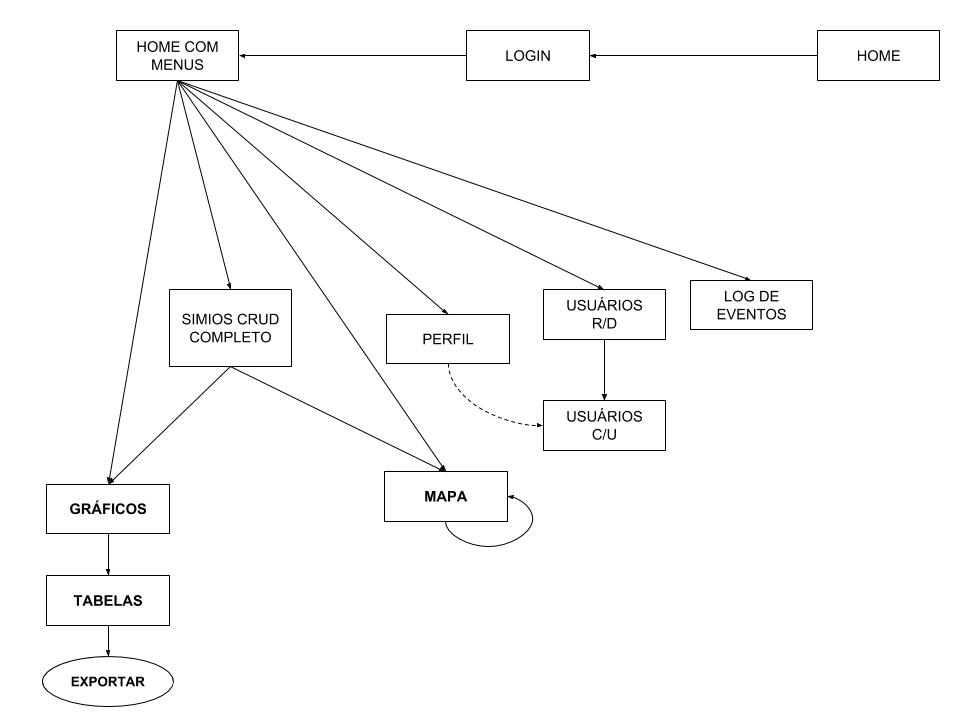
\includegraphics[scale=0.45]{mapa-do-site}
  \centerline{\small{Fonte: autores}}
\end{figure}
\FloatBarrier
